\chapter{Design and Methodology}
\label{cha:methodology}
In this chapter we present the tools and techniques used in our experimental analysis and detail their application. We partition our approach into three categories, each focused on addressing a particular section of our overarching hypothesis. Firstly in \cref{sec:Msimenvironment} we detail the network simulation environment, data sets, and produced tools. In this section we also give a high-level implementation overview of the network, probe paths, and other data structures.\par
Secondly in \cref{sec:Mnetworkprobing} we cover our approach to testing sub-hypothesis one, that network tomography enables inference of node level packet delay metrics within stochastically routing networks. Specifics of how network tomography has been applied and subsequently evaluated w.r.t its ability as a tool to inferring node level metrics are also given.\par
Thirdly in \cref{sec:MNefidentification} we give an overview of our approach to determining router level nefarious hold probability in . In this analysis we identify a novel parametric relationship between router hold probability and packet delay. We then show how this relationship can be inverted to estimate router hold probability from packet delay. Coupled with this we present a secondary approach which requires ground truth metrics of the network known to have no nefarious routers.\par
Finally in \cref{sec:Moptprobing} we segment the complex process of network tomography using a novel representation we refer to as the \textit{tomographic pipeline}. We then cover our implementation of two optimisations to the tomographic pipeline using techniques introduced in \cref{sec:Boptimization}.

\section{Simulation Environment and Tools}
\label{sec:Msimenvironment}
This section details network topology data sets, network traffic data generation, tools for analysis, and developed software packages for evaluation of our overarching hypothesis. Details of data used for real world network analysis are given in \cref{ssec:Mdatasets}. Alterations and additions to the data sets are addressed along with generation of traffic and probing data in \cref{ssec:Mdataprocessing}. Produced packages are listed in \cref{ssec:Msoftware} and implementation details for all classes and analysis scripts can be found in \cite{sylvester_millar_real_2021}.

\subsection{Data Sets}
\label{ssec:Mdatasets}
Real world topology data sets are from the SNDLib project (\cite{orlowski_sndlib_2007}) and the Internet Topology Zoo project (\cite{knight_internet_2011}). We have selected eight national ISP topologies for analysis, details of these network are shown in \cref{tbl:Mrealnetworkattributes}. These topologies were selected as they have a high connectivity (without being fully connected) and large number of nodes (>15) compared to other typologies within the data set. We believe this combination represents real-world scenarios where network tomography can provide useful results with non-trivial performance improvements over conventional monitoring methods.\par
A synthetic 7 router network was also used for initial data exploration. A worked example of network tomography using this network and a diagram of the topology is provided in \cref{sec:Mnetworkprobing}.\par
  \begin{table}
    \centering
    \begin{tabular}{@{}cccccccc@{}} 
      \toprule
      &&&&&\multicolumn{3}{c}{Router Degree}\\
      \cmidrule{6-8}
      Name & Region & Year & \# Routers & \# Links & Min & Max & Mean \\
      \midrule
      Nobel & Germany & 2005 & 17 & 26 & 2 & 6 & 3.05\\
      ACOnet & Austria & 2009 & 23 & 31 & 1 & 8 & 2.7\\
      Free & France & 2005 & 25 & 45 & 2 & 10 & 3.6\\
      CPLEX & Norway & 2005 & 27 & 51 & 2 & 6 & 3.78\\
      Cost266 & Europe & 2005 & 37 & 57 & 2 & 5 & 3.08\\
      Pioro & Poland & 2005 & 40 & 89 & 4 & 5 & 4.45\\
      China Telecomt & China & 2010 & 42 & 66 & 1 & 20 & 3.14\\
      T-Systems & Germany & 2005 & 50 & 88 & 2 & 5 & 3.52\\
      Telekom & Austria & 2005 & 65 & 108 & 1 & 10 & 3.32\\
      \bottomrule
    \end{tabular}
    \caption{Real world network ISP topology attributes.}
    \label{tbl:Mrealnetworkattributes}
  \end{table}

\subsection{Data Processing}
\label{ssec:Mdataprocessing}
Data from both the SNDlib and Internet Topology Zoo projects are stored in a range of bespoke XML and GraphML formats. To maximise speed of the network simulation these formats were parsed into a graph object in the python iGraph library (\cite{csardi_igraph_2006}). Nodes and links from the topology data sets are represented as iGraph vertices and links respectively. All python objects were stored using python's pickle module \cite{van_rossum_python_2020}.\par
An object representing each network device (\textit{i.e. router or switch}) is stored as an attribute of each iGraph vertex along with an id to account for iGraph's dynamic object indexing. Each network device stores an array of packet received each timestep, shuffling and appending elements from this array to its queue buffer to emulate temporal ambiguity in receiving packets. As each packet is an instance of a UDP packet class once the buffer queue reaches capacity additional packets are silently dropped.\par
Despite best efforts network traffic data for systems with robustly mapped topologies and probabilistically delaying routers could not be acquired. Due to this traffic was generated at simulation run time from switches attached to routers. Each switch has a fixed probability of sending a packet with a random destination to its attached router every timestep. As the number of packets received by routers follows a Poisson distribution (see \cref{sssec:Itrafficsimulation}) the number of switches attached to each router is selected at random from the poisson class of numpy's random library.\par
UDP traffic is stochastically routed through the network using a link state (\textit{LS}) protocol. Link state advertisements are broadcast at the start of the simulation and the network is not probed for the first 5\% of the simulation to allow for the routing tables to stabilise. LS advertisements are sent periodically throughout the simulation with path weights to each router representing the sum of router buffer queue length on that path. Routers forward packets to the router with the lowest cumulative path weight.\par
CFR restricted probe paths between monitors are calculated using the \textit{Spanning Tree-Based Path Construction} (STPC) algorithm from \cite{he_network_2021}. Probe paths and linear equations for router identification are stored in a custom format (.dat files within \cite{sylvester_millar_real_2021}) and converted to binary vectors for use in analysis at simulation run time. Probe packet generation is halted before the last 10\% of simulation time to allow probe packets to reach their destination monitor. This emulates real world networks where run time would not be limited and probe packets would be able to traverse the network.\par
To generate robust results 100 subsets of routers are selected iid for each combinations of network attributes in each topology. Each of these sets contains a random number of routers to be designated as nefarious at simulation run time. As the network is stochastically routing all simulation results were then averaged over three 100,000 timestep simulations to minimize variance. All simulation and analysis was conducted on the NCI's Gadi super computer.\par

\subsection{Simulation and Analysis Software}
\label{ssec:Msoftware}
As a result of this work python scripts have been produced for the following functionalities:
\begin{itemize}
    \item Parsing XML/GraphML to iGraph network objects.
    \item Simulating dynamically routing UDP traffic and CFR restricted probe traffic over arbitrary network topologies with nefarious routers.
    \item Parsing network tomography probe paths from and to a custom file format.
    \item Generating a minimal number of CFR restricted probe paths and linear equations to identify router packet delay metrics.
    \item Computing an allocation of probe packets over a set of probe paths to maximise information gain from network tomography.
    \item Classifying nefarious routers under three different sets of assumptions on networking performance logging.
\end{itemize}
Jupyter notebooks were used for initial topology and traffic data exploration as well as visualisation of results. Python scripts were developed using Matplotlib (\cite{hunter_matplotlib_2007}) to produce confusion matrices and receiver operating characteristic plots for evaluation of our classifiers.

\section{Inferring Packet Delay Metrics}
\label{sec:Mnetworkprobing}
In this section we introduce how we have applied additive network tomography to our problem setting.
\begin{mdframed}
\textbf{NOTATION FOR PDV SECTION FORMALIZATION}:\\
Probe path probabilities: Each probe packet is sent along a probe path $p$ with a probability of $\phi_p$, given there are multiple paths within any non-trivial model we represent them all as $\vec{\phi}=\forall p\in P^*, \phi_p$ where $|\vec{\phi}|=|P^*|$, $\phi_p \geq 0$ and $\sum_{p\in P^*}\phi_p = 1$

The parameter vector $\vec{\theta}$ is the vector of length $|R|$ containing the parameter governing each $q\in Q$ where $ q_x \sim \theta_x$ or more formally $\vec{\theta}=\forall r\in R, \theta_r$.

The vector $\vec{\psi}$ is the vector containing all proper path allocations/injection probabilities where $\psi_x$ is the allocation of probes to $p_x\in P^*$ 

Let $f_{Q|\vec{\theta}}(q)$ represent the probability of observing the value $q$ from monitor-to-monitor probe path $p\in P^*$ given the node parameter $\theta_x$ governing $Q_x$.

Note that we can represent a tomographic problem as a system of $P^*f'(\theta)=\mathcal{M}$ where $f'$ is a one-to-one correspondence function of $\theta$ and $\mathcal{M}$ is a matrix of monitor-to-monitor metrics we collect from our probing where $\mathcal{M}_p = (q_1,q_2,\ldots, q_n)$. For ease of notation let $|\mathcal{M}_p|$ be the number of metrics ($n$) we collect over path $p$. Note that for aggregation of measurements after collection $\forall p\in P^*, \forall r\in p, \mathcal{M}=\sum_{r\in p}\theta_r$.
\end{mdframed}
Using Ma's monitor placement algorithm a minimum sufficient subset of routers are designated as monitors. Probe paths between these monitors are then calculated using the spanning tree based construction method from \cite{he_network_2021}. Each probe path is converted to two directed probe paths to allow both monitors on the path to send packets along it. Each directed path is assigned a unique id which is included in the tag field of all probe packets sent along that path. At simulation start probe paths are broadcast from monitors to all routers. Routers store the subsequent router from them on the path as the forwarding destination for any probe packets they receive.\par
The total number of probe packets sent my monitors during analysis can be varied within our simulation tool. We refer to this number of probe packets sent as \textit{probing intensity}. At the end of the simulation the timestep each packet was sent from and received by a monitor is aggregated to give a distribution of packet transmission delays along that path. The average of this distribution is then computed using numpy's vector operation and stored as the path PDA. Path PDA's are then substituted to each router identifiability equation to compute the router level PDA.\par
To validate the accuracy of tomographic probing in a nefarious settings a test was performed on  the seven router network in \cref{fig:M7routersample}. For validation of accuracy the average of 50 simulations with a random set of nefarious routers in each was taken over a range of probing intensities. The average difference between inferred PDA and the true PDA over probing intensities is presented in 
\begin{figure}
    \centering
    \tikzsetnextfilename{7routertopology_methodology}
    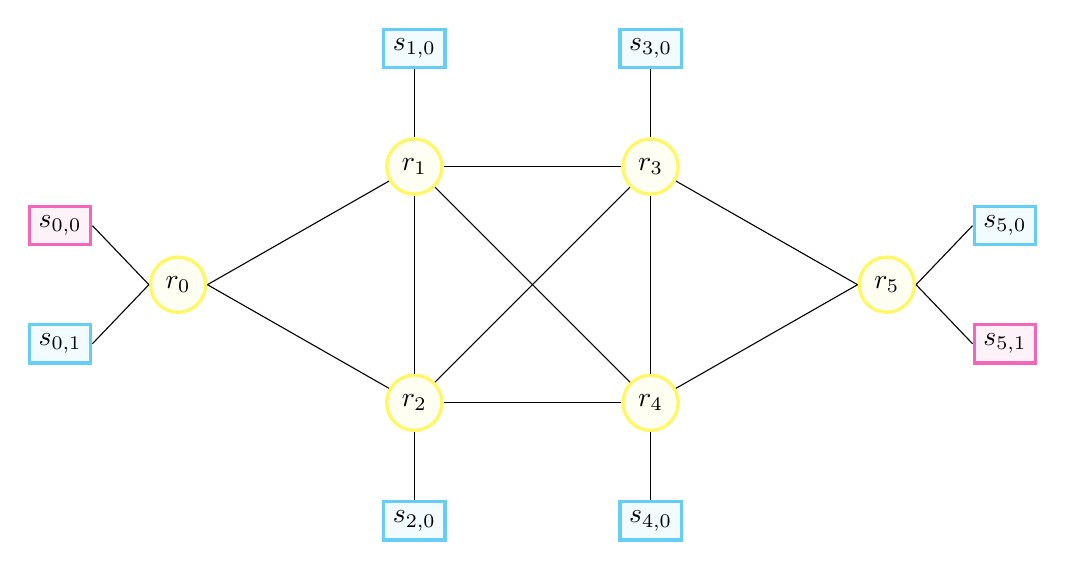
\begin{tikzpicture}[
        router/.style={circle, draw=yellow!60, fill=yellow!5, very thick, minimum size=3.5mm},
        nef_router/.style={circle, draw=red!60, fill=red!5, very thick, minimum size=3.5mm},
        switch/.style={rectangle, draw=cyan!60, fill=cyan!5, very thick, minimum size=2.5mm},
        monitor/.style={rectangle, draw=magenta!60, fill=magenta!5, very thick, minimum size=2.5mm},]
        
        % Routers
        \node[router] (r0) at (-4.5,0)    {$r_0$};
        \node[router] (r1) at (-1.5,1.5)  {$r_1$};
        \node[router] (r2) at (-1.5,-1.5) {$r_2$};
        \node[router] (r3) at (1.5,1.5)   {$r_3$};
        \node[router] (r4) at (1.5,-1.5)  {$r_4$};
        \node[router] (r5) at (4.5,0)     {$r_5$};
        
        %Switches
        \node[monitor](s00) at (-6,.75)   {$s_{0,0}$};
        \node[switch] (s01) at (-6,-.75)  {$s_{0,1}$};
        \node[switch] (s10) at (-1.5,3)   {$s_{1,0}$};
        \node[switch] (s20) at (-1.5,-3)  {$s_{2,0}$};
        \node[switch] (s30) at (1.5,3)   {$s_{3,0}$};
        \node[switch] (s40) at (1.5,-3)   {$s_{4,0}$};
        \node[switch] (s50) at (6,.75)   {$s_{5,0}$};
        \node[monitor](s51) at (6,-.75)   {$s_{5,1}$};
        %Links
        \draw[-] (r0.east) -- (r1);
        \draw[-] (r0.east) -- (r2);
        \draw[-] (r1) -- (r2);
        \draw[-] (r1) -- (r3);
        \draw[-] (r1.south east) -- (r4.north west);
        \draw[-] (r2) -- (r3);
        \draw[-] (r2) -- (r4);
        \draw[-] (r3) -- (r4);
        \draw[-] (r3) -- (r5.west);
        \draw[-] (r4) -- (r5.west);
        \draw[-] (s00.east) -- (r0.west);
        \draw[-] (s01.east) -- (r0.west);
        \draw[-] (s10) -- (r1);
        \draw[-] (s20) -- (r2);
        \draw[-] (s30) -- (r3);
        \draw[-] (s40) -- (r4);
        \draw[-] (s50.west) -- (r5.east);
        \draw[-] (s51.west) -- (r5.east);
    \end{tikzpicture}
    \caption{6 router network with 2 monitors located at $r_0$ and $r_5$ (Reprinted from \pageref{fig:6routersample})}
    \label{fig:M7routersample}
\end{figure}\par

\section{Tomographic Inference}
\begin{figure}[H]
        \centering
        \includegraphics[width=\textwidth]{figs/results/Probe_PDV_accuracy_plot.png}
        \caption{Accuracy of inference from true values over a range of probes sent.}
        \label{fig:Rqstabilization}
\end{figure}

% probe path calculation
% inference accuracy test description


\section{Identifying Nefarious Behaviour}
\label{sec:MNefidentification}
  In our problem setting nefarious behaviour is characterized by a router probabilistically \textit{delaying} packets by not forwarding them during a timestep. As noted in previous chapters we refer to a router's probability of delaying a packet during a timestep as its \textit{hold probability}. To classify a router as behaving nefariously we require a metric that is impacted by this nefarious behaviour and identifiable using network tomography. We postulate that packet delay, serving as a proxy for router buffer queue length, is an appropriate metric. We therefore hypothesise that a router can be classified as exhibiting nefarious behaviour using information gained from packet delay metrics.\par
  This section is divided into three sub-sections, the first two address how we classify nefariously behaving routers and the third how we compare these classifications. \cref{ssec:MTruevalues} covers approaches to classification using the true buffer queue length measurements from routers at simulation time. This is to test our underlying assumption that a routers buffer queue length is influenced by its hold probability. In \cref{ssec:MInferredvalues} we instead use packet delay averages from network tomography to classify routers as nefarious. Following this we present our approach to comparing the classifications using both inferred and true data sets under each case of assumptions.
  
  \subsection{Classification with True Values}
  \label{ssec:MTruevalues}
  In testing our sub-hypothesis we firstly use ground true values of router queue buffer lengths from the simulation. These ground truth values emulate theoretical perfectly accurate results from network tomography. Three approaches to identifying nefarious routers with different additional assumptions are considered. Each additional assumption increases the amount of information available for router classification. The additional assumptions for each approach are:
  \begin{description}
      \item[Case 1:] Known router packet delay metrics with no nefarious routers (\textit{baseline metrics}) and complete distribution of router buffer queue length at each timestep.
      \item[Case 2:] Only known router packet delay metrics with no nefarious routers (\textit{baseline metrics}).
      \item[Case 3:] No additional assumptions.
  \end{description}
  The first set was chosen as it emulates a situation where network tomography yields perfectly accurate results. This serves as a test of whether we are able to accurately classify nefarious routers given full router level information. The second and third sets emulate scenarios where results from network tomographic analysis presented in \cref{sec:Mnetworkprobing} are used for calculation. The second set additionally emulates an system under constant network monitoring. In this scenario metrics with no nefarious routers can be viewed as logged system metrics. The third set represents a scenario where these previous logs are not available or a new system is being analysed.\par
  For cases 1 and 2 we run three additional simulations of each topology with no nefarious routers to serve as baseline metrics. We compute the mean of all metrics from these simulations and use them for our known packet delay metrics with no nefarious routers. With these baseline metrics and results from 500 blind trials with nefarious routers we consider the problem of classification in the case of assumption set 1.\par
  In case 1 we have two distributions of buffer queue lengths for each router with only one known to have been collected from a non-nefarious router. To classify if a router is nefarious using these we assume that a nefariously delaying router will have buffer queue lengths greater than an equivalent non-nefariously delaying router.\par
  To compare these distributions we use SciPy's implementation of a one-tailed two-sample Kolmogorov-Smirnov test (\cite{chakravarti_handbook_1967}) in python. To ensure the classification is accurate we select a p-value of 0.0 as required to classify a router as nefarious. This means we tolerate virtually no chance of the result occurring by chance. We select this extremely low tolerance as our assumptions in this test provide the most information possible. To give a more comprehensive overview of the classifier we produce a receiver operating characteristic (ROC) curve, varying the p-val required to be classified as nefarious.\par
  In case 2 we do not have access to the complete queue buffer length distributions. Instead we use utilise summary statistics obtainable from tomography, specifically PDA and PDV. Without the underlying distribution we are unable to use the Kolmogorov-Smirnov test as in case 1. It follows from our assumption in case 1 that their will be a statistically significant difference in PDA between a nefarious and non-nefarious router.\par
  To account for differences due to noise from stochastic routing we use a standard deviation test for outliers. This test is shown in \cref{eq:stddev} where: $\mu$ and $\sigma$ are the mean and variance of the absolute differences between the baseline and potentially nefarious simulation for all routers, X is the given routers difference from baseline results, and Z is the threshold for being classified nefarious. As in case 1 we vary this threshold for classification as nefarious and present the results using a ROC curve.\par
  
  \begin{equation}
  \label{eq:stddev}
      \frac{\mu-X}{\sigma}>z
  \end{equation}
  
  In the most restrictive scenario of case 3 we have access to neither the underlying router buffer queue distribution nor a baseline of non-nefarious metrics. Therefore to classify a router as nefarious we are required to determine its hold probability from packet delay metrics alone. This is a non-trivial task which we address in depth in \cref{ssec:pdatoholdprob}.\par
  
  % This section could go???
  \subsection{Estimating Hold Probability from Packet Delay Metrics}
  \label{ssec:pdatoholdprob}
  To establish a relationship between router packet delay metrics and hold probability we  consider 100 randomly generated topologies between 10-50 nodes, 50 generated using BA and 50 using ER. Randomly generated topologies are used in-place of the limited number real world topologies to ensure results are robust. We assume that there is an underlying parameterised relationship between a routers hold probability and buffer queue length. With the relationship being parameterised over the two variable network parameters: max buffer queue length and background traffic intensity.\par
  To determine this relationship we simulate each topology with a combinations of max queue length from  200-5,000 and background traffic intensity from 0.1-0.5, each for 10,000 time steps. For each combination of parameters the hold probability of a randomly selected nefarious router is varied from 0.1-0.9. The PDA of the router is recorded along with the corresponding hold probability. Results are then graphed using a scatter plot to visually approximate and display the relationship between these router attributes. For implementation details see \cite{sylvester_millar_real_2021}.\par
  To map an arbitrary hold value to a measured PDA or vice-versa we fit a function to these discrete observed data points. The data is fitted using the curve\_fit function of SciPy's optimize class which we provide an initial guess of parameters. We tested multiple possible function to fit the data but a standard sigmoid function was found to fit best, matching initial visual analysis of the distribution. We provided the curve function with a minimum value of 0 and a maximum of the maximum queue length. The Levenberg–Marquardt minimisation algorithm was used for fitting as it was found to be the best performing of algorithms within SciPy's library. For transparency we present results for curve fitting using Trust Region Reflective and Rectangular Trust Region Dogleg minimisation algorithms in Appendix D.\par
  We record the estimated curve fitting parameters from SciPy's curve fitting, noting the minimum and maximum values are approximately the supplied initial guesses. Finally, variation of the functions parameters w.r.t max queue length and background traffic intensity were modeled. This enabled estimation of the PDA to hold probability relation given only network parameters.\par
  Inverting the observed empirical PDA from varying hold probabilities we are able to estimate hold probability from PDA alone. Using this estimation of hold probability we select a hold probability between 0.0-1.0 as a threshold for a router being classified as nefarious. We then generate a ROC curve to evaluate the efficacy of our classification in the most general context possible. We do not present a confusion matrix  as requirements governing tolerated number of false negatives and false positive will vary between systems.\par
 
  
  \subsection{Classification with Inferred Values}
  \label{ssec:MInferredvalues}
  We combine methods from \cref{sec:Mnetworkprobing} and \cref{sec:MNefidentification} to evaluate our overarching hypothesis that network tomography can be used to identify nefarious routers. This is analogous to cases 2 and 3 from \cref{ssec:MTruevalues}, where summary statistics of router queue lengths are used to classify routers as nefarious. Case 1 is not applicable as the use of an underlying true distribution of router buffer queue lengths can not be obtained with tomography. We cover our method for testing the efficacy of PDA inferred through network tomography as a metric used in identifying nefarious routers firstly under assumption case 2 then 3.\par
  In assumption case 2 where the baseline PDA of each router is known we use the same methods as in \cref{ssec:MTruevalues} to assess if the router is nefarious. From network tomography we have the PDA at each router, analogous to the router's buffer queue length. We then compute the difference between the PDA of the baseline simulation and the simulation with unknown nefarious routers for each router in the network. We use a standard deviation test (\cref{eq:stddev}) to identify routers with a difference between the two simulations larger than a user defined threshold. In assumption case 3 with no baseline metrics to compare against we use solely router level PDA to classify nefarious routers.\par
  For comparison of classifiers under each case of assumptions we consider both a graphic and a numeric presentation of their performance. To evaluate the relative general performance of each method we qualitatively compare the ROC curves produced by each classifier. For a more rigorous quantitative comparison we consider three scenarios covering the spectrum of sensitivity and specificity requirements. Scenario one requires a false negative rate of <2\% and represents a government network with a large budget where compromised routers present a massive risk. Scenario two requires a minimal false positive rate while achieving a false negative rate <25\% and represents a budget restricted cloud provider with quality of service obligations they wish to meet at minimal cost. Scenario three requires a false positive rate of <5\% and represents an organisation monitors a network of honeypot servers intended to be compromised who wants to avoid manual analysis of non-compromised machines.

\section{Optimising Inferential Accuracy}
\label{sec:Moptprobing}
\begin{figure}[H]
    \centering
    \tikzsetnextfilename{tomographicpipeline}
    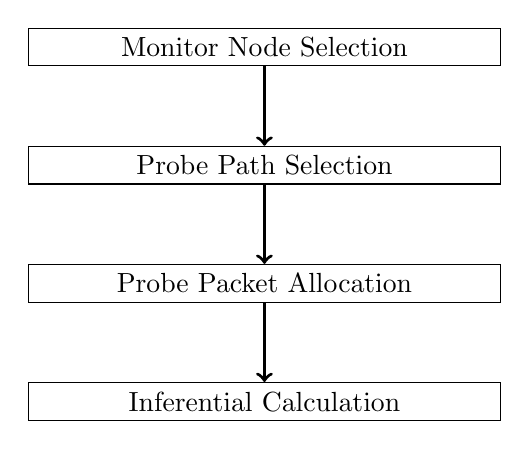
\begin{tikzpicture}
        \node[draw,minimum width=6cm] (A) at (0,4.5) {Monitor Node Selection};
        \node[draw,minimum width=6cm] (B) at (0,3) {Probe Path Selection};
        \node[draw,minimum width=6cm] (C) at (0,1.5) {Probe Packet Allocation};
        \node[draw,minimum width=6cm] (D) at (0,0) {Inferential Calculation};
        
        \draw[->, very thick] (A) -- (B);
        \draw[->, very thick] (B) -- (C);
        \draw[->, very thick] (C) -- (D);
    \end{tikzpicture}
    \caption{The Tomographic Pipeline.}
\end{figure}

\subsection{The Tomographic Pipeline}

\subsection{Parsimonious Probe Path Selection}
\label{ssec:Mpppselection}

\subsection{Probe Allocation}
\label{ssec:Mpallocation}

As probes traversing different nodes and different probes traversing the same node have an independent effect on $q$ we can develop an aggregation of all measurements in $\vec{q}$ assuming $r\in R, q_r \sim \mathcal{N}(0, \theta_r)$ where the variance $\theta_r$ is unknown. Using this this we aim to infer an estimation of $\vec{\theta}$ from our monitor-to-monitor measurements $\vec{q}$. To formalise our knowledge of the network from probing we adapt a standard PDV PMF from \cite{he_network_2021} where $\mathcal{M} = \sum_{r\in p}\theta_r$ in \cref{eq:pdvobservationmodel} and denote the corresponding log-likelihood function as $\widehat{\mathcal{L}}(q, p)$.
\begin{equation}
\label{eq:pdvobservationmodel}
    f_{Q|\vec{\theta},\; \vec{\phi}}(q,\;p) = \phi_p \sqrt{2\pi\mathcal{M}}^{\ q^2/{2\mathcal{M}_r}}
\end{equation}
Using $\widehat{\mathcal{L}}(q, p)$ we are able to represent a network as a FIM, from this the CRB can be posed as a metric representing the lower bound on the accuracy of our inference, we elaborate on the specifics of this representation in \cref{sec:Mnetworkprobing}. Using this CRB however we can show that the equal allocation of probes over paths is a sub optimal approach to probing. Consider the example network in \cref{fig:fimex3routereg} we define three probe paths $p_0$, $p_1$, and $p_3$ traversing $r_0\rightarrow r_2$, $\ r_1\rightarrow r_2$, $\ r_0\rightarrow r_1\rightarrow r_2$, and the reserve directions respectively.
\begin{figure}[H]
    \centering
    \tikzsetnextfilename{3routertopology}
    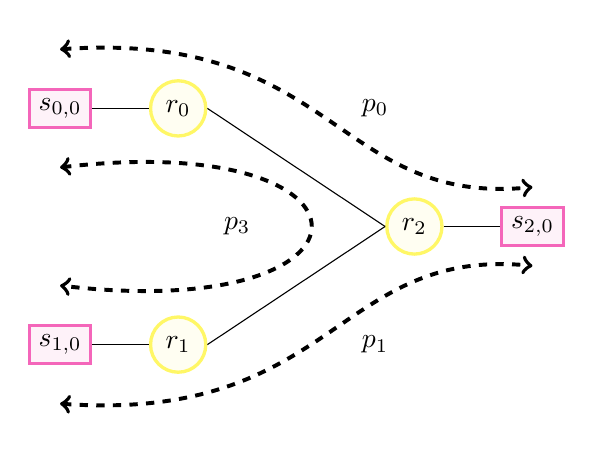
\begin{tikzpicture}[
        router/.style={circle, draw=yellow!60, fill=yellow!5, very thick, minimum size=3.5mm},
        nef_router/.style={circle, draw=red!60, fill=red!5, very thick, minimum size=3.5mm},
        switch/.style={rectangle, draw=cyan!60, fill=cyan!5, very thick, minimum size=2.5mm},
        monitor/.style={rectangle, draw=magenta!60, fill=magenta!5, very thick, minimum size=2.5mm},]
        
        % Routers
        \node[router] (r0) at (-1.5,1.5) {$r_0$};
        \node[router] (r1) at (-1.5,-1.5)  {$r_1$};
        \node[router] (r2) at (1.5,0) {$r_2$};
        %Switches
        \node[monitor](s00) at (-3,1.5)   {$s_{0,0}$};
        \node[monitor](s10) at (-3,-1.5)   {$s_{1,0}$};
        \node[monitor](s20) at (3,0)   {$s_{2,0}$};

        %Links
        \draw[-] (r0.east) -- (r2.west);
        \draw[-] (r1.east) -- (r2.west);
        \draw[-] (r0.west) -- (s00.east);
        \draw[-] (r1.west) -- (s10.east);
        \draw[-] (r2.east) -- (s20.west);
        
        % Probe path visualizations.
        \node at (1,1.5) {$p_0$};
        \draw[dashed, line width=.5mm, <->] (-3,2.25) .. controls (0.5,2.5) and (0.5,0.25) .. (3, 0.5);
        \node at (1,-1.5) {$p_1$};
        \draw[dashed, line width=.5mm, <->] (-3,-2.25) .. controls (0.5,-2.5) and (0.5,-0.25) .. (3, -0.5);
        \node at (-0.75,0) {$p_3$};
        \draw[dashed, line width=.5mm, <->] (-3,0.75) .. controls (1.25,1.25) and (1.25,-1.25) .. (-3, -0.75);

    \end{tikzpicture}
    \caption{Example 3 router network with probe paths explicitly noted.}
    \label{fig:fimex3routereg}
\end{figure}

We examine three different probe allocations between [$p_0,\:p_1$]: $\phi_0$ = [0.33, 0.33, 0.33],  $\phi_1$ = [0.1, 0.8, 0.1], and $\phi_2$ = [0.8, 0.1, 0.1]. As there are no nefarious routers each router has an equal expected true PDV, let these true PDV's be $r_0=1, r_1=1, r_2=1$, the CRB of each probe allocation is then $\phi_0$=2.69, $\phi_1$=5.97, $\phi_2$=5.97. Recalling that the CRB provides a lower bound on inferential accuracy, the equal allocation of probes between paths results in the lowest inferential accuracy, this also holds when nefarious behaviour is included. Suppose the case of $r_1$ being nefarious with a $\frac{1}{3}$ probability of holding a packet any timestep, resulting in an increased PDV of 3 the CRB of each probing scheme is then $\phi_0$=1.51, $\phi_1$=4.24, $\phi_2$=2.05. Although each probing scheme performs worse it is clear that $\phi_0$ is comparatively even worse at detecting the increased PDV of the nefarious router than the case of no nefarious nodes. Note for comparison that in the previous case of being $r_1$ nefarious a pseudo optimal probing allocation $\phi_{optimal}$ = [0.0, 0.5, 0.5] results in a CRB of 33.67.

\section{Summary}
\todo{Once chapter is finished recap what we showed with a reference to each section.}
